% !TEX root = main.tex
\chapter{序論}
\section{研究背景}
\subsection{半導体レーザー}
\subsubsection{半導体レーザーの現状}
半導体レーザーが実現されたのは1962年のことである 。キャリアと光の閉じ込めを能率よくできるようにした2重ヘテロ構造が用いられるようになり実用化・発展を遂げた。光通信、光ディスク用発光デバイスの核をなす技術である。他のレーザー\delspan{に}と比較しても小型・軽量、大量生産可能、熱や振動(安定性)に強いことなどが主な理由である。近年では半導体からピコ秒程度の超短光パルスを発生させる技術も研究が盛んに行われており、産業への応用が期待されている。
%[利得スイッチングsds生物発光yokoyamaさん,ここではGSにこだわらなくてもいいか][psパルスを使った産業]

\subsubsection{半導体レーザーの基礎特性}
\addspan{半導体レーザーの定常発振条件について述べる。}
ここで半導体レーザーの特性について説明する。
まずは発振条件について述べる。
発振条件は共振器の中を往復する光が共振器を1周したときに元の光強度と同じであることである。これは式で表すと単位長さあたりの光損失$\alpha$ (/cm)、誘導放出による利得$g$ (/cm)、端面での反射率R(2つの端面の反射率を同じとした)を用いて
\begin{eqnarray}
\sqrt{R}\sqrt{R} \rm{exp}(-2\alpha L+ 2gL-i2\beta L)=1
\label{eq:1}
\end{eqnarray}
と書ける。Lは共振器長である。$\beta$は伝搬定数である。
この条件を満たす利得すなわち閾値利得は
\begin{equation}
g_{\rm{th}}=\alpha+\dfrac{1}{L}\rm{ln}\left(\dfrac{1}{R}\right)
\end{equation}
と書ける。また式(\ref{eq:1})の虚部が0になるという条件から
\begin{eqnarray}
2\beta L=2\pi m   (mは整数)
\end{eqnarray}
を得る。伝搬定数を2$\pi n_{\rm{eq}}/\lambda$と表すと、共振波長は
\begin{eqnarray}
\lambda =2n_{\rm{eq}}L/m
\end{eqnarray}
となる。$n_{\rm{eq}}$は光分布全体で空間積分した等価屈折率である。

次にキャリアの再結合時間$\tau(n)$はバンド間の発光再結合寿命$\tau_{r}(n)$と非発光再結合寿命と$\tau_{nr} (n)$を用いて
\begin{eqnarray}
\dfrac{1}{\tau}=\dfrac{1}{\tau_{r}}+\dfrac{1}{\tau_{nr}}
\label{eq:tau_r}
\end{eqnarray}
で与えられる。$1/\tau_{n}$と$1/\tau_{nr}$はそれぞれ\addspan{発光再結合と非発光再結合の}割合であるから、内部量子効率$\eta_{int}$は全\delspan{キャリアの}再結合のうちの発光再結合の割合\delspan{であるから}\addspan{として}
\begin{eqnarray}
\eta_{int}=\dfrac{1/\tau_{r}}{1/\tau_{r}+1/\tau_{nr}}
\end{eqnarray}
で表される。
\subsubsection{超短パルス発生}
ピコ秒オーダーの超短パルスを発生する技術は長距離光ファーバー伝送\cite{ref_hasegawa}に加えて、精密レーザー加工\cite{ref_chichkov} や多光子励起顕微鏡を用いたバイオイメージングなど、応用の幅が広がってきている技術である。
%\addspan{領域}である。

半導体レーザーを用いた短パルス発生の代表的な方法としては利得スイッチングとモード同期法がある。利得スイッチング\cite{ref_h_ito}は注入電流を変調する直接変調の一種である。デバイスにナノ秒程度の電流パルスを注入すると励起パルスよりも短い、数十psの光パルスが得られるというものである。半導体内の光強度が大きくなると誘導放出によって利得が急激に減少するためである。特徴としては複雑な構造を必要とせずほとんどの半導体レーザーで実現可能な技術であるという点である。

一方のモード同期法はサブps程度の超短パルスを得ることができる技術である。外部共振器あるいは共振器内に過飽和吸収体を挿入するなど付加的な構造が必要となる。

本研究では\delspan{比較的容易に実現できる}\addspan{半導体キャリアの高速ダイナミクス物理により直結した}利得スイッチングに注目する。
\begin{comment}
 半導体から短パルスを発生させる方法として従来行われてきた方法が主に3つある。モード同期法、Qスイッチ法、利得スイッチ法である。モード同期法は個体レーザーでも用いられておりフーリエ限界に近いパルス幅を生成できる反面パルスの繰り返し周期が固定されてしまうという特徴を持つ。一方Qスイッチング法は過飽和吸収帯を用いるなどしてQ値を瞬間的に増大させることで高エネルギーの光パルスを得ることができる。利得スイッチングは電流を変調する直接変調の一種であり、複雑な構造を必要とせず、全ての半導体レーザーで実現が可能な技術である。レーザー加工などの技術的応用においては繰り返し可変であることや様々な種類の光源を試すことができるという利点があるため、??本研究では利得スイッチング法に着目した。
\end{comment}


\subsubsection{利得スイッチング法}
利得スイッチングは1980年ごろに観測された\cite{ref_h_ito}\cite{ref_aspin}\cite{ref_torphammar}。光通信技術向上を念頭に置いた高周波変調技術の研究のなかで短パルス光が確認された。ItoらはAlGaAsレーザーに閾値以下のDCバイアスと100$\sim$300MHzの高周波変調を重層することで時間幅約30 ps光パルスが発生できることを報告した。その後電源として用いるパルスジェネレーターの進歩などにより研究が進み報告も盛んに行われてきた。
約5 psの非常に短い報告もなされている\addspan{\cite{ref_nagarajan}}。\adsp02{Chenらは1.55 \si{\micro\metre}波長帯において電流注入利得スイッチングパルスの高周波成分を切り出すことで4.7 psのパルス幅の実現を報告している\cite{chen_yokoyama}。}
%図\ref{fig:fig_1_1_GS_ito}bに過去40年間に報告されてきた利得スイッチングのパルス幅がプロットされている。赤が光励起、青が電流注入を表している。電流注入の報告を見てみると最短でも5ps程度である。

また応用としては利得スイッチングを利用した生物発光イメージの撮像の報告がある\cite{ref_h_yokoyama}。


次に利得スイッチングの基本的な動作について述べる。


利得スイッチング\adsp02{の基本}動作は半導体中のレーザー動作特性を記述する\adsp02{シングルモード}レート方程式により理解されている\cite{ref_lau}。
レート方程式はデバイス中のキャリア密度と光子密度の時間変化の振る舞いを以下のような連立方程式で表している。$ n$ は量子井戸1層あたりのキャリア密度、$s$ は全活性層の光子密度を表す。式(\ref{eq:late_eq_1})は$ n$ の時間変化を記述している。右辺第1項は外部から注入されるポンプキャリア、第2項は誘導放出、第3項は自然放出を表す。式(\ref{eq:late_eq_2})は光子の時間変化を記述しており、第1項は誘導放出による増幅、第2項は光子寿命による減衰(共振器寿命)、第3項は自然放出光を表す。
\begin{eqnarray}
\dfrac{dn}{dt}&=&n_{\rm{pump}}\zeta(t)-\dfrac{\Gamma}{m}\nu_{\rm{g}}g(n)\dfrac{s}{1+\epsilon s}-\dfrac{n}{\tau_{r}}\\
\label{eq:late_eq_1}
\dfrac{ds}{dt}&=&\Gamma\nu_{g}g(n)\dfrac{s}{1+\epsilon s}-\dfrac{s}{\tau_{p}}+m\beta\dfrac{n}{\tau_{r}}
\label{eq:late_eq_2}
\end{eqnarray}
\begin{eqnarray*}
&n& : 量子井戸1層あたりのキャリア密度 [\rm{m^{-3}}]\\
&s& : 活性層全体の光子密度[\rm{m^{-3}}]\\
&n_{\rm{pump}}& : 励起キャリア密度 \\
&\zeta(t)& : 規格化された励起パルスの時間変化\\
&\Gamma & : 光閉じ込め係数\\
&m& : 量子井戸数\\
&\nu_{g}& : 群速度[\rm{m/s}]=c/n_{eq}\\
&g(n)& : 利得[\rm{cm^{-1}}]\\
&\epsilon & : 利得圧縮係数\\
&\tau_{r}& : キャリアの発光再結合寿命[\rm{s^{-1}}]\\
&\tau_{p}& : 共振器寿命 [\rm{s^{-1}}]\\
&\beta& : 自然放出光係数\\
\end{eqnarray*}
共振器寿命$\tau_{p}$はファブリー・ペローレーザーの場合
\begin{eqnarray}
\tau_{p}=\dfrac{n_{\rm{eq}}}{c(\alpha+\rm{ln}  (1/\it R)/L)}
\label{eq:tau_p}
\end{eqnarray}
とかける\cite{ref_iga}。
$n_{\rm{eq}}$は等価屈折率、$\alpha$は共振器内部の損失、$c$は光速、$L$は共振器長、$R$は共振器のミラー端面の反射率である。
\begin{comment}
\subsubsection{半導体レーザーの特性}
半導体レーザーの基本的な特性について説明する。
まずは発振条件について述べる。
発振条件は共振器の中を往復する光が共振器を1周したときに元の光強度と同じであることである。\delspan{これは}式で表すと単位長さあたりの光損失$\alpha$ (/cm)、誘導放出による利得$g$ (/cm)、端面での反射率R(2つの端面の反射率を同じとした)を用いて
\begin{eqnarray}
\sqrt{R}\sqrt{R} \rm{exp}(-2\alpha L+ 2gL-i2\beta L)=1
\label{eq:1}
\end{eqnarray}
と書ける。Lは共振器長である。$\beta$は伝搬定数である。
この条件を満たす利得すなわち閾値利得は
\begin{equation}
g_{\rm{th}}=\alpha+\dfrac{1}{L}\rm{ln}\left(\dfrac{1}{R}\right)
\end{equation}
と書ける。また式(\ref{eq:1})の虚部が0になるという条件から
\begin{eqnarray}
2\beta L=2\pi m   (mは整数)
\end{eqnarray}
を得る。伝搬定数を2$\pi n_{\rm{eq}}/\lambda$と表すと、共振波長は
\begin{eqnarray}
\lambda =2n_{\rm{eq}}L/m
\end{eqnarray}
となる。$n_{\rm{eq}}$は光分布全体で空間積分した透過屈折率である。

次にキャリアの再結合時間$\tau(n)$はバンド間の発光再結合寿命$\tau_{r(n)}$と非発光再結合寿命と$\tau_{nr}(n)$を用いて
\begin{eqnarray}
\dfrac{1}{\tau}=\dfrac{1}{\tau_{r}}+\dfrac{1}{\tau_{nr}}
\label{eq:tau_r}
\end{eqnarray}
で与えられる。$1/\tau_{n}$と$1/\tau_{nr}$はそれぞれ割合であるから、内部量子効率$\eta_{int}$は全キャリアの再結合のうちの発光再結合の割合であるから
\begin{eqnarray}
\eta_{int}=\dfrac{1/\tau_{r}}{1/\tau_{r}+1/\tau_{nr}}
\end{eqnarray}
で表される。
\end{comment}
%\subsubsection{利得スイッチング}
上式のようなレート方程式を基に短い励起パルスを印可した時の発光および利得の時間変化についてシミュレーションを行った結果を図\ref{fig:fig_1_1_GS_ito}aに示す。赤線が光励起によるインパルス励起の様子、青線が電流注入による数 ns秒パルス励起の様子である。青線に注目すると図\ref{fig:fig_1_1_GS_ito}a上段での励起パルスよりも短い、数十 ps光パルスが出てくることがわかる。さらに1つ目のパルスの後は緩和振動が起きている。これが典型的な利得スイッチング動作である。また下段には利得の時間変化が示されている。励起が始まると同時に電子密度つまり利得が増えていき、ある時刻をすぎると閾値に達し反転分布を形成する。今度は誘導放出によって一気にキャリアが消費される。このキャリアの消費が注入されるキャリアよりも大きくなるため、利得も急激に減衰し光パルスも光子寿命程度で立ち下がる。これが利得スイッチングの大まかな理解である。

\begin{figure}[h]
	\centering
	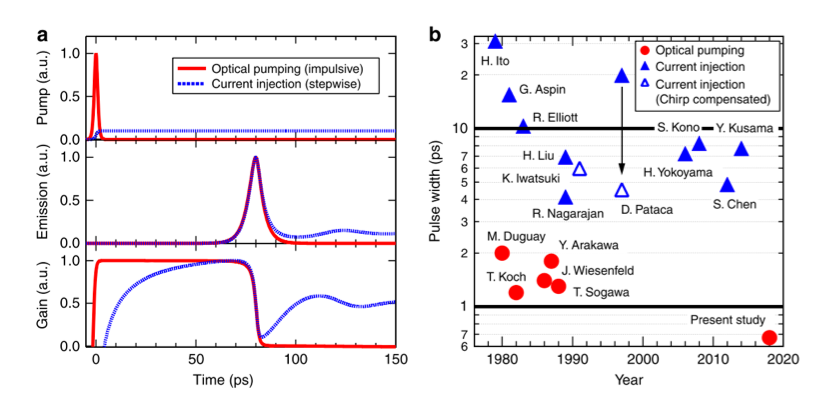
\includegraphics[width=15cm]{figure/fig_1_1_GS_ito.png}
	\caption{a 利得スイッチングのメカニズム, b過去の研究におけるパルス幅\cite{ref_t_ito}}
	\label{fig:fig_1_1_GS_ito}
\end{figure}

\newpage
\subsubsection{利得スイッチングパルスの詳細な理解}
利得スイッチング光パルスのより詳細な理解を視覚的に表したのが図\ref{fig:fig_1_1_GS_pulse}である\cite{ref_1_1_GS}である。
\begin{figure}[ht]
	\centering
	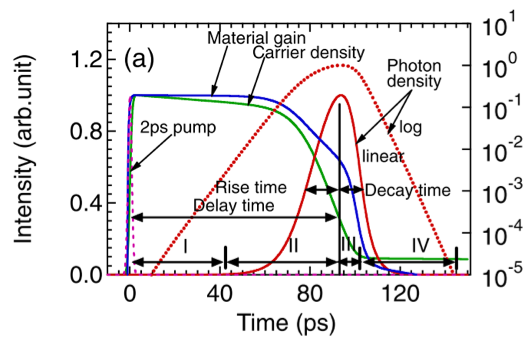
\includegraphics[width=15cm]{figure/fig_1_1_GS_pulse.png}
	\caption{パルス生成中のキャリア密度、光子密度、材料利得の時間変化\cite{ref_1_1_GS}}
	\label{fig:fig_1_1_GS_pulse}
\end{figure}

レート方程式の誘導放出の項に関わってくる材料利得$g(n)$はキャリア密度$n$に比例する線形利得$g_{0}(n-n_{0})$のような形で近似されてきた($g_{0}$は利得定数,$n_{0}$は透明キャリア密度)。しかしChenらは$g(n)$に非線形な項を取り入れたシミュレーションを行った。利得を式(\ref{eq:nonlier_gain})のように記述した。線形な項に加えて$g_{s}$といった利得飽和の効果を取り入れている。図\ref{fig:fig_1_1_GS_pulse}にこの時のパルス生成中のキャリア密度、光子密度および利得の時間変化を表す。時刻0で2 psのインパルス励起行った時の光の時間波形赤の実線と破線、キャリア密度を緑の線、材料利得を青い線で表している。
\begin{eqnarray}
\label{eq:nonlier_gain}
g(n)&=&g_{0}(n-n_{0})\left[1+\dfrac{g_{0}(n-n_{0})}{g_{s}}\right]^{-1}\\
&\simeq &\left\{
\begin{array}{ll}
 g_{0}(n-n_{0}) & n-n_{0}\ll g_{s}/g_{0}\nonumber \\
g_{s} & n-n_{0}\gg g_{s}/g_{0}\nonumber
\end{array}
\right.
\end{eqnarray}
するとIとIIの領域つまり立ち上がりの時間領域では光子密度が小さい一方でキャリア密度が大きいため、$g_{s}$が支配的に立ち上がりのはやさの限界を決めている。IIIの領域ではキャリア密度が減少し、光強度が大きい領域では$\epsilon$が効いてくる。IVの領域ではキャリア密度も光子密度も小さくなっているため減衰の速さは光子の共振器寿命$\tau_{p}$によってきまる。

つまり利得スイッチングパルスのパルス幅は立ち上がりのはやさを\delspan{利得飽和}\addspan{飽和モード利得}$\Gamma g_{s}$、立ち下がりのはやさを共振器寿命$\tau_{p}$が決めている。
\newpage

\subsubsection{利得スイッチングパルスの短パルス化}
利得スイッチングパルスの短パルス化のためには\delspan{利得飽和}\addspan{飽和モード利得}$\Gamma g_{s}$を大きくすることと共振器寿命$\tau_{p}$を短くすることが必要であると示唆された。
\begin{comment}


共振器寿命$\tau_{p}$はファブリー・ペローレーザーの場合
\begin{eqnarray}
\tau_{p}=\dfrac{n_{\rm{eq}}}{c(\alpha_{a}+\rm{ln}(1/R)/L)}
\label{eq:tau_p}
\end{eqnarray}
とかける\cite{ref_iga}。
$n_{\rm{eq}}$は等価屈折率、$\alpha_{a}$は共振器内部の損失、cは光速、Lは共振器長、Rは共振器のミラー端面の反射率である。
\end{comment}
\addspan{式}(\ref{eq:tau_p})を見ると$\tau_{p}$を小さくするためには端面反射率$R$を小さくすること\addspan{あるいは}共振器長$L$を短くなるようレーザー設計することが有効であるとわかる。
通常端面反射率を下げるためにはためには誘電体膜をコーティングする手法が用いられる。コーティングは光の高出力化のためにも用いられている一般的な手法である。


\delspan{この段落大きく変えた}


\begin{comment}
\delspan{利得飽和}\addspan{飽和利得}$g_{s}$は\addspan{単層の活性層}\delspan{用いる}材料によって決定されるパラメータである\delspan{ためデザインの段階で決めることはできない。そこで式(\ref{eq:late_eq_2})の第1項、誘導放出の項に注目してみると$g(n)$の代わりに}\addspan{一方で$\Gamma$は全体の構造によって決まる。}を大きくすることが有効であるとわかる。\addspan{モード利得}$\Gamma g(n)$を大きくすることができるためである。$\Gamma$が大きくなるような\delspan{結晶}\addspan{全体}構造をデザインすることが利得スイッチングパルスの短パルス化につながる。\addspan{本研究では伊藤らが行った\cite{ref_t_ito}ような飽和利得$g_{s}$の領域については考えず、光閉じ込め係数$\Gamma$を増大させることによるモード利得$\Gamma g$の増大について考える。}
%多重量子井戸にすることと$g_{s}$には関係があるんだっけ?ない
%このように利得スイッチングには興味深い非線形性が含まれており詳細に理解を進めることは半導体レーザーそのものの理解にも繋がりうる。
\addspan{飽和利得}$g_{s}$は単層の活性層材料によって決定されるパラメータである。一方光閉じ込め係数$\Gamma$はウエハ全体の構造によって決定される。
\end{comment}
\addspan{飽和利得$g_{s}$は量子井戸の活性層材料によって決定されるパラメータである。一方光閉じ込め係数$\Gamma$はウエハ全体の構造によって決定される。本研究では伊藤ら\cite{ref_t_ito}が光励起実験で示した飽和利得$g_{s}$の影響が現れるような領域については考えず、光閉じ込め係数$\Gamma$増大させることによるモード利得$\Gamma g$の増大について考える。}
\clearpage
\subsection{InGaAs高利得材料}
先の節で\addspan{モード利得を大きく}\delspan{高利得化}することによ\delspan{る}\addspan{り}利得スイッチングパルスの高速化が見込めることについて述べた。

本節では量子井戸レーザーにおける多重量子井戸化を\delspan{持ちた}\addspan{用いた}高利得化について述べる。合わせて多重量子化の結晶成長の\delspan{の}際に生じる結晶の歪みについても述べる。
\subsubsection{量子井戸レーザー}
まず量子井戸レーザーであるが
%井戸の中の電子のエネルギーが離散値をとるので発振波長の短波長化が図れる(どうでもよくない?)
、閾値電流密度の温度変化が小さい(バンド端の状態密度が大きいことに由来)、再結合効率が大きい(キャリアが量子井戸に閉じ込められることに由来)などの特徴を有する。


量子井戸レーザーは1975年Van der ZielらによってMBEにより作られた\cite{ref_van}。DupuisらはMOCVD法により量子井戸レーザーの作製を行い閾値電流の温度依存性が量子井戸レーザーでは抑えられることなどを指摘した\cite{ref_dupuis}。%T_{0}がでかい
MBEやMOCVDの発展により様々な材料の量子井戸レーザーが作られている。
%閾値電流密度が実現され注目を集めたのち、
%その後Tsangにより$0.25kA/cm^{2}$の程閾値電流密度をもつ量子井戸レーザーが発表され注目を集めた。近年では様々な材料の量子井戸レーザーが作られている。
\subsubsection{多重量子井戸レーザー}
量子井戸レーザーの特徴の1つとして量子井戸の厚さ、量子井戸の数のデザインが可能である、という点があげられる。ここで量子井戸の数mに注目する。単一量子井戸とm周期多重量子井戸を比較した場合、透明電流はm倍になる反面、第一サブバンドに収容できるキャリアの数がm倍になるためモード利得(光閉じ込め係数$\Gamma$×材料利得$g$)もm倍になることが予想される。
%しかしこれは材料利得が線形であることを想定した場合であり、利得の平坦化を考えると図のようにgが変化することが計算されている。[]目指す利得によって適切な井戸数を選ぶ必要があることを示唆している。

m周期多重量子井戸レーザーと単一量子井戸レーザーを比較した場合を考える。
半導体レーザーの発振条件は誘導放出の\addspan{モード}利得\delspan{(光閉じ込め係数 × 材料利得)}が全体の損失に等しいというものであるから、
%\begin{eqnarray}
%\Gamma g_{mod}=\alpha^{total}= \xi a_{\rm{ac}} +(1-\xi)a_{\rm{ex}}+\rm{ln}(1/R)/L
%\end{eqnarray}
\begin{eqnarray}
\label{eq:th}
\Gamma g_{\rm{material}}&=&\alpha^{\rm{total}}= \Gamma \alpha_{\rm{ac}} +(1-\Gamma)\alpha_{\rm{ex}}+\dfrac{1}{L}\rm{ln}\left( \dfrac{1}{\it R} \right )\\
&=& \alpha + \dfrac{1}{L}\rm{ln}\left( \dfrac{1}{\it R} \right )
%\Gamma g_{\rm{material}}=\alpha^{\rm{total}}= \alpha +\dfrac{1}{L}\rm{ln}\left( \dfrac{1}{R} \right )
\end{eqnarray}

と書ける。
$\alpha_{\rm{ac}}$はキャリアが注入される活性層(active layer)の損失、$\alpha_{\rm{ex}}$はクラッド層およびバリア層の損失の平均を表す。
$L_{z}$を量子井戸の厚さ、光波の実効的な広がりの厚さを$L_{0}$とすると、$L_{z}\ll L_{0}$の場合光閉じ込め係数$\Gamma$は近似的に
\begin{equation}
\Gamma = mL_{z}/L_{0}
\label{eq:Gamma}
\end{equation}
と書ける。$L_{0}$は典型的に0.1umである。
一方注入電流については
\begin{equation}
J_{m}=J_{m=1}
\label{eq:J_M}
\end{equation}
という関係がある。注入電流密度はキャリア面密度Nを用いて
\begin{equation}
J_{m=1}=eN/\tau_{r}
\end{equation}
と表せる。式(\ref{eq:J_M}はm周期多重量子井戸はm倍のモード利得が得られることを意味する。その反面発振に必要な注入電流もm倍になる。(透明電流密度)単一量子井戸の材料利得が注入電流と線形な関係にあると仮定すると、つまり
\begin{eqnarray}
g_{\rm{material}}=a(J_{m=1}-J_{g})
\end{eqnarray}
と書けるならば($J_{g}$は透明電流密度,aは係数)単一量子井戸レーザーの閾値電流は式(\ref{eq:th})と式(\ref{eq:Gamma})より
\begin{eqnarray}
J^{\rm{th}}_{m=1}&=&\alpha^{total}/ a\Gamma + J_{g}\nonumber\\
&=&\alpha^{total}/(aL_{z}/L_{0})+J_{g} 
\end{eqnarray}
と書ける。また多重量子井戸レーザーでは式(\ref{eq:J_M})より
\begin{equation}
J_{m}^{t\rm{h}}=\alpha^{totla}/(aL_{z}/L_{0}) + mJ_{g}
\label{eq:Mj0}
\end{equation}
となる。常に単一量子井戸レーザーの方が低い閾値電流を与えることになる。これは材料利得が注入電流に対して線形な場合の結論である。実際には励起強度を上げていくと(つまり擬似フェルミ準位を増加させていくと)サブバンド端では利得が飽和する。


図\ref{fig:fig_gain_mode}に量子井戸層の数を変えたときのモード利得と注入電流の関係を示す\cite{y_arakawa}。横軸が注入電流、縦軸がモード利得である。電流が小さいときには井戸数が少ない方がモード利得が大きい。しかし電流を大きくしていくと井戸数が多い方が高いモード利得を得られることがわかる。
 %モード利得が共振器の正味の損失$\alpha^{\rm{total}}$に等しくなると発振を開始する。そのため、$\alpha^{\rm{total}}$が大きいようなデバイスにおいては多重量子井戸構造の方が高いモード利得を得られるため閾値電流を下げるのには有利である。また電流量を増やしていくと
\begin{figure}[h]
	\centering
	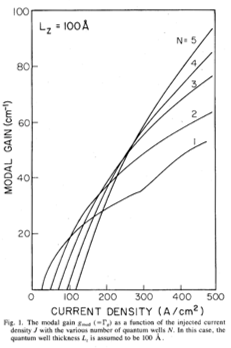
\includegraphics[width=5cm]{figure/fig_1_1_gain_mode.png}
	\caption{量子井戸層の数を変えたときのモード利得と注入電流の関係}
	\label{fig:fig_gain_mode}
\end{figure}


%モード利得のずほしい


%言いたいこと
%要は多重にするとモード利得が大きくなるため高速化に適している。

\subsubsection{量子井戸レーザーにおける歪効果}
前節で多重量子井戸化することで高利得を実現できることを述べた。
しかし活性層とバリア層の結晶格子定数が異なる場合歪が発生してしまう。このため量子井戸を\delspan{無限に}厚く積むことはできない。
本節ではこの歪による多重量子井戸レーザーの性能の変化の紹介と多重量子井戸化における歪の影響について述べる。
歪量子井戸は活性層とバリア層あるいはクラッド層の結晶格子定数に違いにより歪が発生することを利用している。層の厚さが数nmの薄膜になると内部に歪を含んだままミスフィット転移を起こさずにを膜を成長させることができ歪量子井戸を作ることができる。
\begin{figure}[h]
	\centering
	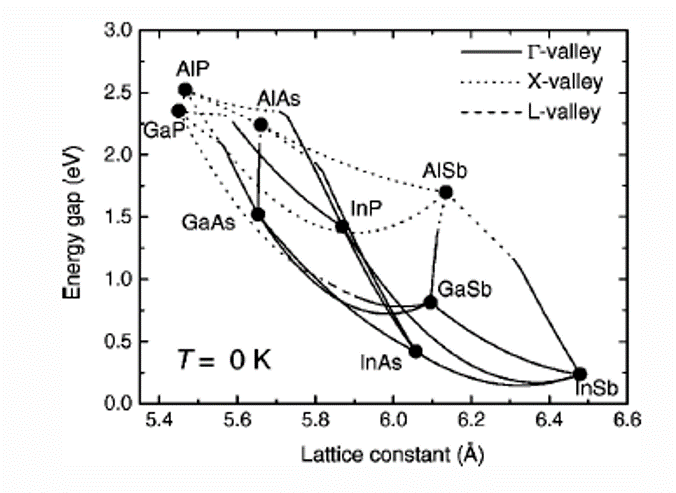
\includegraphics[width=14cm]{figure/fig_1_1_lattice_constance.png}
	\caption{III-V族原子の格子状数とバンドギャップの関係\cite{ref_band_para}}
	\label{fig:fig_1_1_lattice_constance}
\end{figure}

一般にヘテロ\delspan{結合}\addspan{構造材料}においては格子定数が異なる。
図\ref{fig:fig_1_1_lattice_constance}にIII-V族原子の格子状数とバンドギャップの関係を示す\cite{ref_band_para}。例えばGaAsの格子定数は5.65\AA 、 InAsの格子定数は6.06\AA と0.4\AA 程度大きいことがわかる。またInGaAsに関してもGaAsよりも格子定数が大きい。InGaAsをGaAsの上に結晶成長させようとした場合、格子定数の大きいInGaAsがどのように歪むかを図\ref{fig:fig_lattice_strain02}に模式的に示す。井戸方向については圧縮され、積層方向については引っ張られるように変形する。
ヘテロ界面に平行な井戸方向の面内歪を$\epsilon_{\|}$、垂直な歪を$\epsilon_{\bot}$とした。

基板の格子定数をa、 活性層の格子定数を$a+\Delta a$とすると
歪は
\begin{eqnarray}
\epsilon_{\|}&=&\epsilon_{xx}=\epsilon_{yy}=-\dfrac{\Delta a}{a}\\
\epsilon_{\bot}&=&\epsilon_{zz}=-\dfrac{2C_{12}}{C_{11}}\epsilon_{\|}\simeq -\epsilon_{\|}
\end{eqnarray}
と書ける。$\epsilon_{\|}<0$が圧縮歪、$\epsilon_{\|}>0$が引っ張り歪に対応する。$C_{11}$と$C_{12}$は弾性定数と呼ばれる値で通常正四面体結晶構造の半導体では$C_{11}\simeq 2C_{12}$の関係が成り立つ\cite{ref_iga}。


このとき体積変形(静水圧変形)と軸方向変形の合成を見ると
\begin{eqnarray}
\epsilon_{\rm{vol}}&=&\Delta V/V=\epsilon _{xx}+\epsilon _{yy}+\epsilon_{zz}\simeq \epsilon_{\|}\\
\epsilon_{\rm{ax}}&=&\epsilon_{\bot}-\epsilon_{\|}=-\dfrac{C_{11}+2C_{12}}{C_{11}}\epsilon_{\|}\simeq 2\epsilon_{\|}
\end{eqnarray}
と書ける。
\begin{figure}[h]
	\centering
	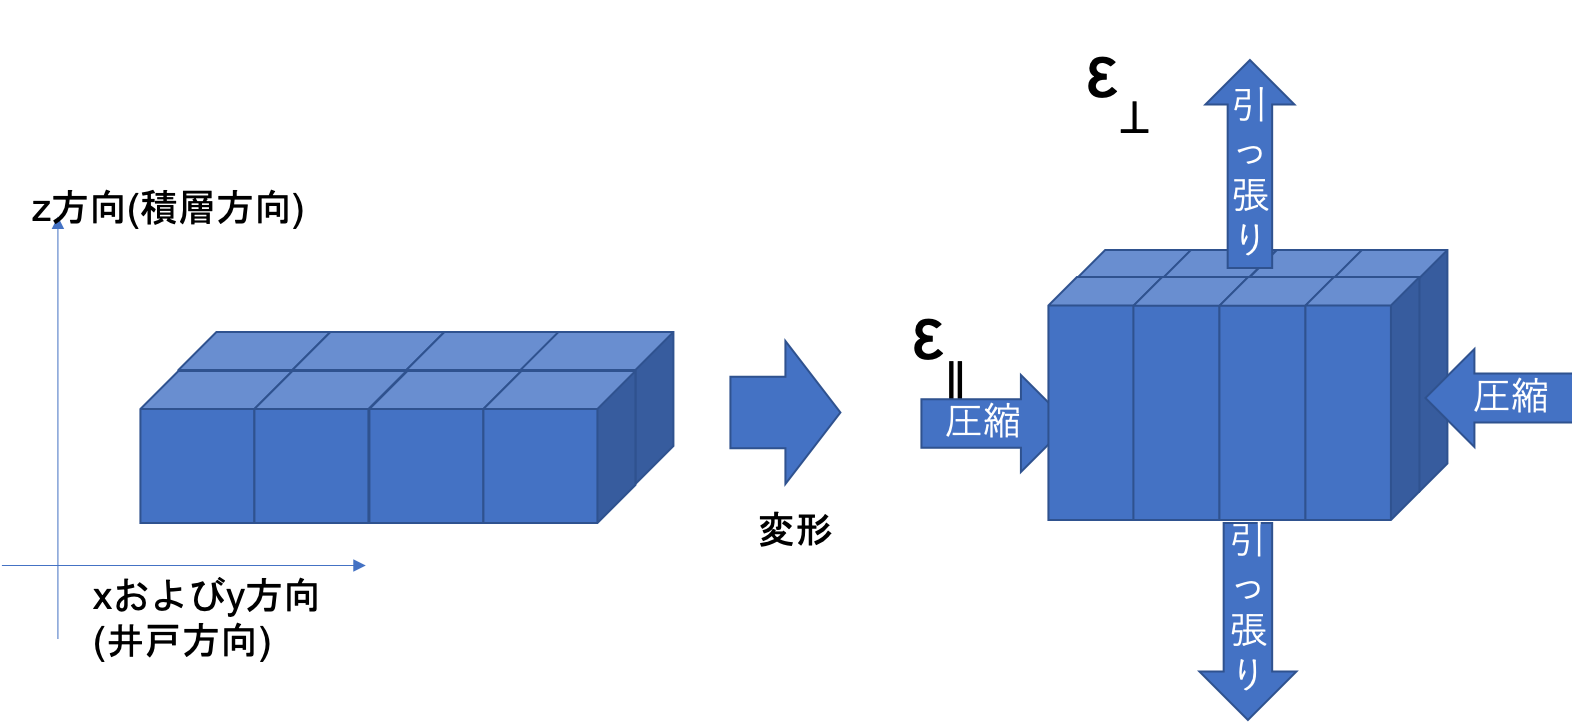
\includegraphics[width=10cm]{figure/fig_1_1_lattice_strain02.png}
	\caption{歪の模式図}
	\label{fig:fig_lattice_strain02}
\end{figure}
歪みの発生により結晶内部に応力エネルギーが蓄えられる。このエネルギーが転移の発生に必要なエネルギーを超えなければ結晶は安定となる。応力エネルギーは膜厚に比例するため転位が発生しない最大の膜厚が存在する。これを臨界膜厚と呼ぶ。

図\ref{fig:fig_1_2_strain_vs_d}にInGaAs/GaAs歪超格子のInGaAs層における歪と膜厚、結晶性の関係を示す\cite{ref_konagai}。実線は理論的に導かれた臨界膜厚である。プロットはフォトルミネッセンスおよびホール測定などにより結晶性を調べたもので、黒プロットは高品質と判断されるもの、白抜きプロットは結晶性が劣ると判断されるものである。これらを見ると実験と理論がよく一致しており臨界膜厚以上の厚さでは結晶の品質が低下することがわかる。

\begin{figure}[h]
	\centering
	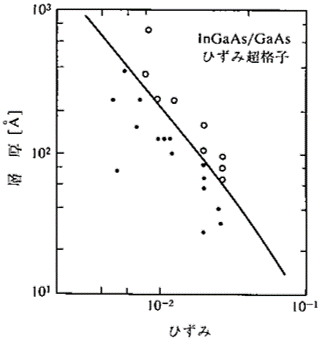
\includegraphics[width=10cm]{figure/fig_1_2_strain_vs_d.png}
	\caption{InGaAs/GaAs歪超格子のInGaAs層における歪と膜厚、結晶性の関係}
	\label{fig:fig_1_2_strain_vs_d}
\end{figure}
\begin{comment}
Matthewsらは多重薄膜構造において転移の発生しない限界の層厚$H_{c}$を理論的に次のように導いている。\cite{ref_Matthews}
\begin{eqnarray}
h_{c}=\dfrac{b(1-\nu \cos ^2 \alpha)}{2\pi f (1+\nu ) \cos \lambda}\left(\rm{ln}\dfrac{h_{c}}{b}+1\right)
\end{eqnarray}

ここで$b=a\sqrt{2}$、$f=2\epsilon$、$\nu$ : ポアソン比、$\alpha$ : 転移線とバーガースベクトスのなす角、$\lambda$ : すべり面と海面の光線に垂直な面の方向をすべり面の方向のなす角である。
\end{comment}

次に歪みがある場合のバンド構造の変化およびそれが及ぼすレーザー特性について定性的に述べる。

体積変形歪みは伝導帯と価電子帯のバンド端をシフトさせバンドギャップ$E_{g}$を$\Delta E_{g}=a\epsilon_{\rm{vol}}$だけ変化せさせる。aは静水圧変形ポテンシャル(hydrostatic deformation potential)と呼ばれる定数である。GaAsでは2.7 eV、InAsでは2.5 eV報告されている\cite{ref_adachi}。一方軸性変形歪は価電子帯の構造を変化させ、量子井戸レーザーの特性変化の主要因となっている。歪がない半導体では価電子帯の頂上はヘビーホールとライトホールが縮退しているが、軸性歪により縮退が解けてそれぞれの頂上が上下反対方向にシフトする。バンドの分離量は$E_{ll-hl}\simeq -2b\epsilon_{\rm{ax}}$で与えられる。bは軸性変形ポテンシャルと呼ばれる。


%ここに$k_{\|}$方向の図ほしい

圧縮歪の場合、一番上の量子化準位の$k_{\|}$方向のバンド構造はライトホールになっている。すると有効質量が小さく、すなわち状態密度が小さい。するとキャリア注入による擬フェルミ準位の変化が大きくなり反転分布が生じやすくなる。(反転分布の条件:$E_{fc}-E_{fv}>h\omega _{p}\geq E_{g}$を達しやすくなる)したがって発振閾値が無歪に比べて小さくなる。引っ張り歪の場合準位間分離が大きくなると価電子帯混合の影響が減って$k_{\|}$方向の有効質量が小さくなる。これにより閾値を下げることが可能である。光ファイバ通信用の1.55um帯で低い閾値電流密度が報告されている\cite{ref_thijs}。図\ref{fig:fig_lattice_strain_Ith}に歪の異なるレーザーについての閾値電流密度を共振器長の逆数に対してプロットした図を示す。この報告の中ではInP基板の上に$\rm{In_{x}Ga_{1-x}As}$を結晶成長させたレーザーを用いている。引っ張り歪みが0, 1.1, 1.5, 2.2の単一量子井戸レーザーについて歪が大きいほど閾値電流が低くなることを報告した。
\begin{figure}[h]
	\centering
	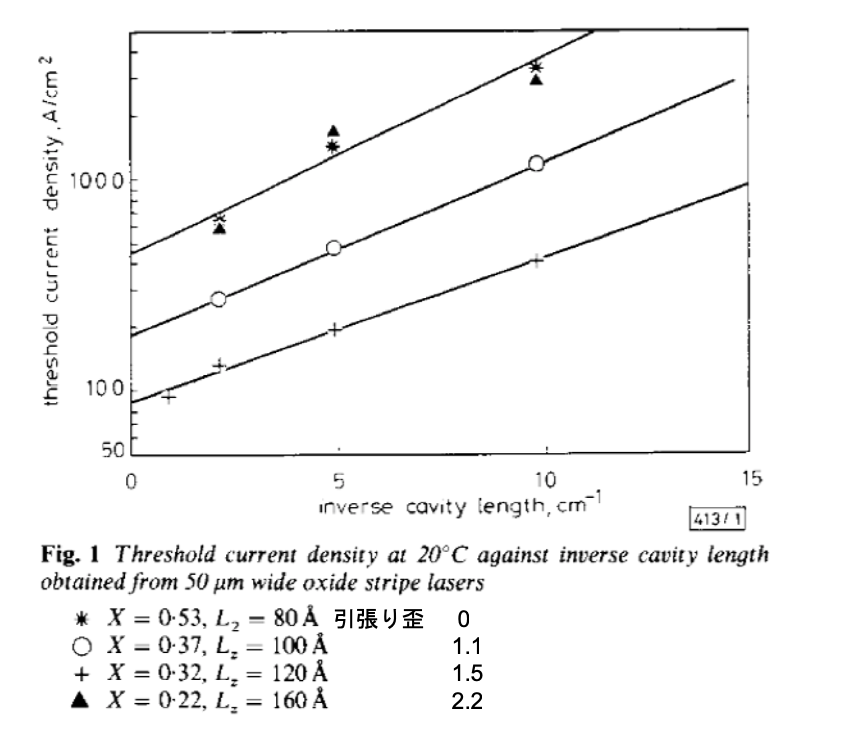
\includegraphics[width=10cm]{figure/fig_1_1_lattice_strain_Ith.png}
	\caption{単一歪み量子井戸レーザーの閾値電流密度\cite{ref_thijs}}
	\label{fig:fig_lattice_strain_Ith}
\end{figure}

%じゃあ3QWの利得計算してみれば?ってなるよね
\clearpage
\subsubsection{InGaAs歪補償レーザー}
%式(\ref{eq:Gamma})からわかるように多重量子化することで光閉じ込め係数を増大させ正味の利得を増やすことができる。
多重量子井戸化を行うにも格子不整合による歪が生じるために井戸層を積むことのできる限界の厚さが存在することを前節で述べた。


井戸層の歪をバリア層で補償する歪補償量子井戸が導入された。図\ref{fig:fig_1_1_lattice_constance}の格子定数とバンドギャップの関係の図を見ると、InGaAsはGaAsよりも格子定数が大きく、GaAsPは小さいことがわかる。GaAsに格子整合する際に\rm{InGaAs}層とGaAsP層をnmスケールで交互に結晶成長することで\rm{InGaAs}に生じる圧縮歪をGaAsPに生じる引張り歪で相殺しながら結晶成長することができる。
歪補償の条件は以下の式で表される。井戸層の格子定数および厚みを$a_{well}$、$L_{well}$、バリア層の格子定数と厚みを$a_{barrier}$、$L_{barrier}$とする。
\begin{eqnarray}
<a>=\dfrac{a_{well}L_{well}+a_{barrier}L_{barrier}}{L_{well}+L_{barrier}}=a_{substrate}
\label{eq:conpensate}
\end{eqnarray}
格子整合の模式図を図\ref{fig:fig_1_1_lattice_strain_comp}に示す。このように格子整合を行うことで量子井戸数を増加させることが可能になる。


歪補償により微分利得の増加の報告もある\cite{ref_Dutta}。DuttaらはInGaAs/GaAs系3周期歪量子井戸レーザーとInGaAs/GaAsP系4周期歪補償量子井戸レーザーの線形利得をそれぞれ$dg/dn$=1.0$\times 10^{-15}\rm{ cm^{2}}$と$dg/dn$=2.1$\times 10^{-15}\rm{ cm^{2}}$と見積もっている。

歴史的には歪補償を行うことにより発光スペクトルおよび吸収スペクトルの長波長化も目的とされていた。
%歪み補償は\cite{ref_t_kawamura}
%歪み補償の説明→歪み補償を使ったレーザー→高利得のレーザー作った人いるかな
%どういう目的今まで歪補償レーザーが作られてきたのか?
%(温度特性300K以上の閾値電流の温度依存性の小さいレーザーが実現された[T.Hayakawa])余裕があったら入れる
%g_{0}が大きくなることを言cちゃダメかも
%Yb ドープファイバーで増幅可能な波長帯域
\begin{figure}[h]
	\centering
	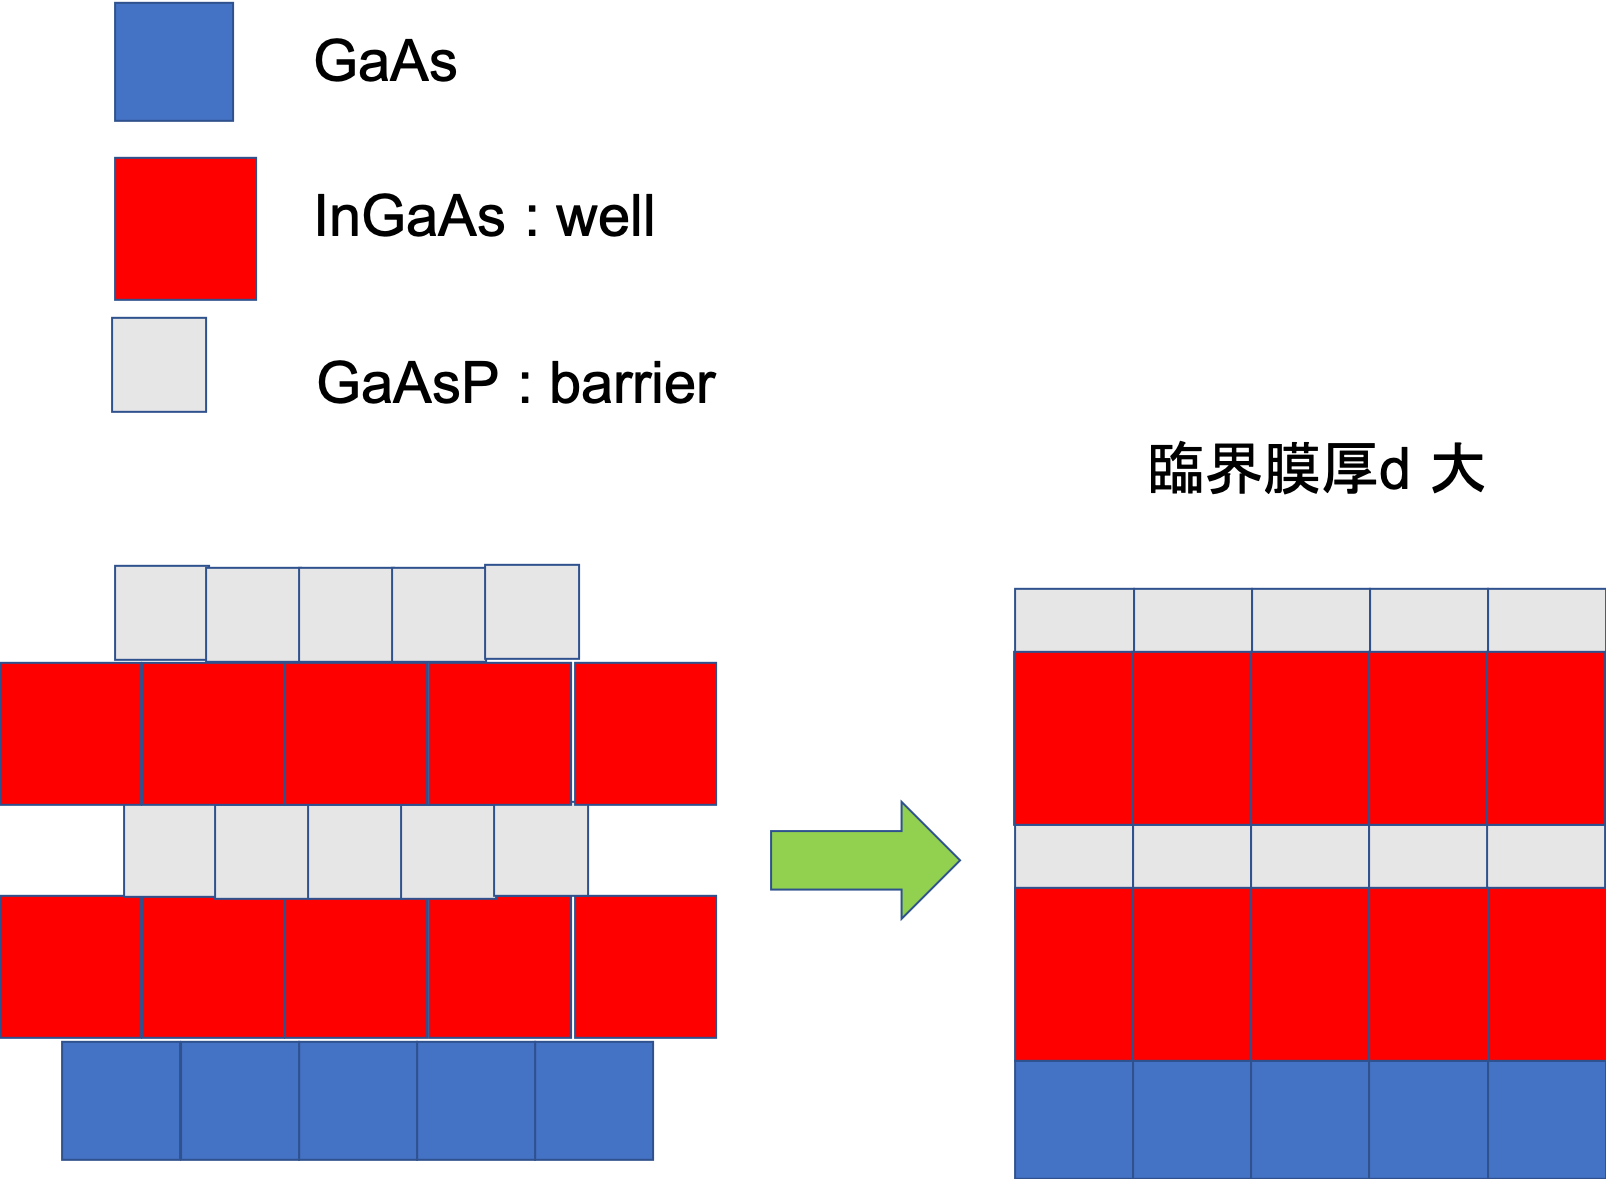
\includegraphics[width=10cm]{figure/fig_1_1_lattice_strain.png}
	\caption{格子整合の模式図}
	\label{fig:fig_1_1_lattice_strain_comp}
\end{figure}
%N.K.Duttaらは歪補償4周期InGaAs/GaAsPレーザーで$\Delta g/\Delta n =2.1 \times 10^{-15}$というそれまでのレーザーよりも高い値を報告している。また。歪み補償があるものとないもので変調感度が3dB低下する周波数が似た構造のレーザーでそれぞれ32GHz、35GHzと報告している。
%もしかして10周期ってめっちゃ多い?

\section{本研究の目的}
\begin{comment}
電流注入による直接変調を利用した利得スイッチングは従来より超短パルス発生の手法として用いられてきた。レート方程式により利得スイッチングパルスのメカニズムが説明され、短パルス化の要因として共振器長Lを短くし共振器寿命$\tau_{p}$を短くすること、およびモード利得$\Gamma g$を大きくすることが必要であると理解されてきた。特にモード利得の増大に着目すると、量子井戸の多重化による光閉じ込め係数$\Gamma$の増大の優位性も示された。

多重量子井戸化に関しては、InGaAsを井戸層としてGaAsに格子整合を行う場合にはGaAsPが歪補償のためのバリア層として有効である。

そこで本研究では多重量子井戸InGaAs/GaAsP材料を用いたレーザーデバイスをデザイン、作製することを目的とする。さらに作製した試料に対して電流注入実験を行う。デバイスのレーザー特性、特に量子井戸の多重化によるモード利得の増大が見られるかどうかを調べる。また利得スイッチング動作を試み過去の報告に匹敵する短パルス発生が可能かを推し量ることも目的とする。
%過去の報告よりもさらに多い10周期歪補償量子井戸レーザーの作製を行いさらなる短パルス化を目指す。
\end{comment}


\addspan{\adsp02{本研究では}
応用上重要な電流注入型の1\si{\micro\metre}波長帯InGaAs系半導体レーザーの利得スイッチング動作に注目する。GaAs材料を用いた光励起による測定実験については以前より研究室でも研究がなされ、利得スイッチングパルスのメカニズムについて説明がされてきた。しかしInGaAs材料、電流注入については先行研究\adsp02{や}参考例が少ないため基礎物理に立ち戻って設計・計画・評価測定を行いフィードバックする必要がある。}


\addspan{利得スイッチングパルスの短パルス化は、共振器長$L$を短くし共振器寿命$\tau_{p}$を短くすること及びモード利得$\Gamma g$を大きくすることで図れることが示されてきた。
光閉じ込め係数$\Gamma$の増大がモード利得$\Gamma g$の増大に寄与する。}


\delsp02{特にモード利得に着目すると量子井戸の多重化による光閉じ込め係数の増大の優位性も示唆されている。}\delsp02{多重量子井戸に関して、InGaAsを井戸層としてGaAsに格子整合を行う場合はGaAsPをバリア層として用いることが有効である。}


\addspan{
\adsp02{本研究では量子井戸レーザーにおいて光閉じ込め係数$\Gamma$の増大は量子井戸の層数を増やすことで実現されることに着目し多重量子井戸半導体レーザーのデザイン及び開発を行う。InGaAs系材料の格子定数はGaAs材料の格子定数よりも大きい。そのためInGaAs系材料をGaAs基板に格子整合を行いながら、層数を多くすることは格子欠陥が生じるなどの品質低下をまねきやすい。そこでGaAsよりも格子定数の小さいGaAsPをバリア層に用いることでInGaAs/GaAsP系10周期歪補償量子井戸レーザーを作製する。}}

\adsp02{電流注入では光励起と異なり電子と正孔の密度を活性層に等しく注入できるか否かは自明ではない。よって多重量子井戸の層数を増やすことで単純に高利得化を実現できるとは限らない。比較のために歪補償を行わずに結晶成長させたInGaAs/GaAs系3周期歪量子井戸レーザーの試作も行う。}
\delsp02{本研究ではこれらのことを踏まえ、InGaAs/GaAsP多重量子井戸材料を用いたレーザーデバイスをデザイン・試作・作製することを目的とする。具体的には10周期歪補償量子井戸レーザーと3周期歪量子井戸レーザーを作製する。さらに}
\delsp02{
作製した試料に対して電流注入評価測定を行う。定常電流注入実験を通してデバイスのレーザー特性を評価し、量子井戸の多重化によるモード利得の増大の有無を調べる。}


\adsp02{レーザーデバイスの作製後、定常電流注入実験を行い閾値電流及びスロープ効率の見積もりを行う。これらの値を解析することでモード利得を算出する。10周期歪補償量子井戸レーザーと3周期歪量子井戸レーザーのモード利得を比較し、期待される量子井戸多重化の効果の有無を調べることも目的とする。}

\addspan{また短パルス電流注入実験を行い利得スイッチング動作を試みる。量子井戸の多重化または共振器長を短くすることによる、光パルスの短パルス化が実現されるかどうかの評価測定を行うことも目的とする。}

